\documentclass[11pt]{article}

% Page layout
\usepackage[margin=1in]{geometry}

% Spacing
\usepackage{setspace}
\onehalfspacing

% Encoding and fonts
\usepackage[utf8]{inputenc}
\usepackage[T1]{fontenc}

% Packages
\usepackage{graphicx}
\usepackage{tabularx}
\usepackage{threeparttable}
\usepackage{multirow}
\usepackage{url}
\usepackage{hyperref}
\usepackage{float}
\usepackage{natbib}
\usepackage{authblk}

\title{Nobel Prize}

\author[1,2,3,*]{Chad M.\ Topaz}
\author[2]{Arden Fleuhr}
\author[1,4]{Jude Higdon}
\author[2]{Anvi Kurongonayini}
\author[5]{Ariana Mendible}
\author[2]{Bennett Ptak}
\author[6]{Rachel Roca}
\author[3]{Nancy Rodr\'{i}guez}
\author[2]{R\'{e}gan Schwartz}
\author[7]{Lu Xian}

\affil[1]{QSIDE Institute}
\affil[2]{Williams College}
\affil[3]{University of Colorado--Boulder}
\affil[4]{Bennington College}
\affil[5]{Seattle University}
\affil[6]{Michigan State University}
\affil[7]{University of Michigan}
\affil[*]{Corresponding author: chad.topaz@gmail.com}

\begin{document}

\maketitle

\begin{abstract}
We did a project.
\end{abstract}

\section{Introduction}
\label{sec:introduction}

Within the academic community, few awards compare in professional and public prestige to the Nobel Prize. Alfred Nobel was a 19th-century scientist and inventor who amassed a fortune from the invention of dynamite and the manufacturing of armaments. Perhaps prompted by his labeling in the press as ``the merchant of death'' \citep{Gol2000}, he endowed the eponymous prizes, meant to honor ``those who, during the preceding year, have conferred the greatest benefit to mankind'' in the areas of chemistry, physics, physiology or medicine, literature, and peace \citep{NobelPrizeWebsiteFull}.

The first Nobel Prizes were awarded in 1901, and as of 2020, there were 962 winners, or \emph{laureates}. The vast majority of these are men \citep{LunJenJau2019} and most express geographic origin in Europe or North America \citep{Fisher2013}. More generally, a substantial body of research identifying the overrepresentation of individuals who are white, men, cisgender, heterosexual, and/or nondisabled has brought into stark relief the degree to which minoritized individuals in certain fields must fight against exclusion in order to participate \citep{TopSen2016, TopKliBer2019, LarTay2020, ACTReport, TopHigEpp2022}. Why might this matter?

Lack of diversity and inclusion through the vertical tiers of an academic or professional field is problematic for several reasons. First, intersectional diversity can create more inclusive and more strategic thinking that compounds into broader diversity and inclusion \citep{exp2021,ACTReport,HunLayPri2015}. Additionally, diverse representation can help ensure that a professional culture and the products that emerge from it, be they physical or digital products, knowledge, services, or anything else, will be designed and executed not only to avoid harm to marginalized individuals but, ideally, to serve as a corrective factor to help address historic inequity \citep{ACTReport,WilMilKas2021}. Finally, there is a huge benefit achieved when individuals from marginalized groups look at high levels of a field and see people with whom they share identity characteristics that contribute to marginalization. When they see more professionally advanced people who have a seat at the table, it bolsters their ability to imagine themselves in such positions in the future and prompts the creation of and works towards ambitious goals \citep{OysBybTer2006, WilMilKas2021}.

\subsection{Previous Work}

An existing body of work has examined Nobel Laureates and their demographics. For example, \citet{BafVam2011} investigate the ages of laureates and \citet{ChaEllRah2011} delve into gender, demonstrating that women laureates are less likely to marry or have children as compared to men. Perhaps unsurprisingly, laureates are overwhelmingly white, male, and affiliated with a university \citep{Cra2001}. Furthermore, many nominees come from only a few countries; for example, between 1901 to 1951, three-quarters of physics nominees came from the US, Britain, Germany, and France, while none came from the continent of Africa \citep{Cra2001}. Laureates enjoy a range of benefits such as more citations of their work, more freedom to focus on their work, increased funding, and global publicity \citep{CasFan2013}. Indeed, \citet{WagHorWhe2015} find that laureates produce fewer papers than matched peers but with higher average citations, and that laureates occupy more central positions in coauthorship networks, suggesting that recognition and network centrality reinforce one another.

Arguably, identifying who has \textit{not} won a Nobel Prize is a richer line of questioning and one that has been around since the prize's conception. In terms of gender biases, the lack of women in STEM fields does not account fully for the low number of female laureates; with strong confidence, women are under-represented \citep{LunJenJau2019}. \citet{ModGilSha2018} trace the long-standing gendered barriers in scientific recognition, documenting how women scientists have historically been excluded from nomination despite demonstrable contributions. The very conditions needed for Nobel Prizes have also excluded and created conflict from its conception. For example, the rule that only three individuals can share a prize for a given advancement erases invaluable work done in collaboration with more scholars. The exclusion of certain collaborators has caused several controversies throughout the years, as listed by \citet{CasFan2013} and \citet{Led2016}. Only living scientists may be awarded a Nobel Prize, which puts the onus on recognizing individuals for their contribution before they are disqualified by death. Several collaborators did not share Nobel Prizes for their contributions for this very reason \citep{CasFan2013}. Beyond gender, \citet{NeiVueVue2024} examine racial and national disparities among laureates in physiology or medicine, finding stark underrepresentation of Black scientists and highlighting persistent gaps in data reporting on ethnicity, gender identity, and disability that limit intersectional analysis.

%human decision-making, different levels
Nobel prizes are awarded to those ``conferred the greatest benefit on mankind,'' \citep{nobelwill}, but choosing who has made the most important contribution is a subjective and inevitably biased choice that greatly depends on those with direct participation in the process. Depending on the scientists who compose the selection committee (discussed more later), preferences of theoretical or experimental work may account for why scientists with clear support never won a prize \citep{But2016, Cra2001}. Some areas of study were not recognized as sub-fields of the larger categories from the prizes' conception, such as astronomy in physics \citep{CasFan2013}. Further, lack of broad international support, grudges, and previous awards in similar areas of study all affect who wins the award \citep{But2016}. But the committee is not the only way bias can enter the Nobel system. \citet{BafVam2011} highlight this nuance by writing ``if there is a preference for older Nobel candidates, this is introduced during the nomination process.'' \citet{GalDom2019} use network analysis to show that nominations are shaped by homophily, with nominators tending to favor individuals from similar national and institutional backgrounds, and that nominees endorsed by central, prestigious actors are more likely to become laureates. \citet{KoJanYan2024} further demonstrate that national favoritism, or ``particularism,'' pervades the nomination process, with wealthy nations disproportionately nominating their own citizens and political, economic, and colonial factors influencing recommendations independently of scientific merit.

%In 1974, some of the secrecy surrounding the process was alleviated when the Nobel Foundation decided to release information regarding nominees and nominators 50 years after the prize was given. While this information has been invaluable in both the above studies and our work, it is probable that contenders will not be alive to have an understanding of the process. A number of factors are still unknown to the public even after the 50 years. For example,

%using networks
\citep{MolIniRui2021, HanSch2021, GalDom2019, ChaZhaPan2017, CasFan2013}

%Lu: I'm working on it!
Papers to discuss might include \citep{ChaFu2021,ChaZhaPan2017,GalDom2019,HanSch2021,LiRouLia2022,MolIniRui2021,Nature2022,NdlMarSha2018,SzeMaSin2018,UrdGre2015,Rod2022}

\subsection{Nobel Prize Selection Process}

Nobel Prize selection processes are complex and opaque. One reason for the lack of clarity is that there appears to be no definitive scholarly source, and indeed no single source at all, with a complete description of these processes. We now aim to fill this surprising gap in the literature. The discussion that follows draws from online sources, namely the websites of the \citet{NobelPrizeWebsiteFull}, the \citet{RSAS}, the \citet{KINA}, and the Wikipedia entry for the Nobel Peace Prize \citep{NPPWiki}.

Table~\ref{Tab1} summarizes relevant actors for the selection of the five Nobel Prizes. Here, we focus on the individuals who wield influence on the process, and so we do not include nominees and laureates in the table. We begin with a general discussion of the various actors and, subsequently, proceed to a more detailed discussion for each specific Nobel Prize.

\newcolumntype{s}{>{\raggedright\arraybackslash} p{0.15\textwidth}}
\begin{table}[t!]
\footnotesize
\begin{threeparttable}
\caption{Overview of the process for selection of Nobel Laureates. For each Nobel Prize, a governing body chooses from among a group of potential vetters in order to create a vetting body. The vetting body receives nominations made by nominators and creates a short list of viable laureates. The selection body takes the vetting body's input and makes the final choice of laureate.\label{Tab1}}
\bigskip
\begin{tabular}{p{0.12\textwidth}sssss}
               & \bf Chemistry                                          & \bf Physics                                            & \bf Physio/Med                             & \bf Literature                           & \bf Peace                                                      \\ \cline{2-6}
               &&&&& \\
\bf Governing Body & Royal Swedish Academy of Sciences                  & Royal Swedish Academy of Sciences                  & Nobel Assembly at Karolinska Institutet               & Swedish Academy                      & Storting\tnote{1}                                                   \\
&&&&&\\
\bf Potential Vetters    & Royal Swedish Academy of Sciences                  & Royal Swedish Academy of Sciences                  & Karolinska Institutet                                & Swedish Academy                      & Norwegian politicians\tnote{2} \\
&&&&&\\
\bf Vetting Body   & Nobel Committee for Chemistry\tnote{3}                      & Nobel Committee for Physics\tnote{3}                        & Nobel Committee for Physio/Med                & Nobel Committee for Literature\tnote{3}       & Norwegian Nobel Committee                                  \\
&&&&&\\
\bf Nominators     & By invitation based on stated eligibility criteria & By invitation based on stated eligibility criteria & By invitation based on stated eligibility criteria & Based on stated eligibility criteria\tnote{4} & Based on stated eligibility criteria                       \\
&&&&&\\
\bf Selection Body & Royal Swedish Academy of Sciences                  & Royal Swedish Academy of Sciences                  & Nobel Assembly at Karolinska Institutet                & Swedish Academy                      & Norwegian Nobel Committee \\ \\ \cline{2-6}
\end{tabular}
\bigskip
\begin{tablenotes}
\item[1] The Storting is the Norwegian parliament.
\item[2] It is not a formal eligibility requirement to be a politician, nor to be Norwegian. However, the Storting has stated that ``As far as possible, the composition of the Committee is to reflect the relative strengths of the political parties in the Storting.'' Moreover, historically, all members of the committee have indeed been Norwegian.
\item[3] Five members of the Vetting Body are chosen by the Governing Body, and then several additional members of the Vetting Body are added by the Vetting Body itself; these are called \emph{co-opted} members.
\item[4] Similar to the Vetting Bodies for Chemistry, Physics, and Physiology/Medicine, the Vetting Body for Literature does send out letters soliciting nominations. However, unlike for those other prizes, for the Literature prize, individuals who meet certain eligibility requirements can nominate even if they did not receive a letter of invitation to do so.
\end{tablenotes}
\end{threeparttable}
\end{table}

Each prize has a \emph{governing body} that oversees the nomination and selection processes. This governing body chooses from among \emph{potential vetters} to create a \emph{vetting body}. The vetting body is in charge of soliciting and/or receiving nominations. \emph{Nominators} are the individuals who nominate candidates for the different awards.  For three of the five awards, individuals who meet certain criteria can become nominators only by invitation of the vetting body. For the other two awards, \emph{any} individual who meets the stated criteria for eligibility can nominate. After receiving nominations, the vetting body sends out nominee portfolios to experts (who do not appear in the table) for evaluation, assesses the nominees, and suggests a shortlist of possible laureates to the governing body. This \emph{governing body} makes the final selection of laureate(s).

Each specific Nobel Prize selection process has unique nuances. The prizes with the most similar processes are the Nobel Prizes in Chemistry and Physics. The governing body for both awards is the Royal Swedish Academy of Sciences (RSAS), established in 1739 as an independent organization to promote the influence of science across the globe. New members are elected by current members. Today, the RSAS has about 480 Swedish and 175 foreign members, divided by discipline into ten classes. The Nobel Committees for Chemistry and Physics are the vetting bodies, respectively, for the prizes. Each committee is made up of five voting members from the relevant RSAS class. The first task of the vetting body is to send out forms to qualified individuals asking for nominations. Typically, each committee receives 250 - 300 nominations. Eventually, based on externally solicited evaluations and its own deliberations, each committee prepares a report with a list of finalists. During the final selection meeting of the RSAS, all present members of the RSAS discuss the report and vote on a finalists. One to three candidates are selected each year for each prize.

The Nobel Prize in Physiology and Medicine involves different actors. The governing body is the Nobel Assembly at the Karolinska Institutet, which is a medical research institute in Sweden. Since 1984, the Nobel Assembly is composed of 50 members of that institute. The vetting body is the Nobel Committee for Physiology or Medicine and consists of five voting members appointed by the Nobel Assembly from among the Karolinska Institute. The selection body, which chooses the laureate(s), is the Nobel Assembly.

The Nobel Prize in Literature is governed by the Swedish Academy (not to be confused with the RSAS). The Swedish Academy is composed of 18 members who are appointed for life.  The Nobel Committee for Literature, the vetting body, is selected from among the members of the Academy for a three-year term.  While the vetting body sends letters to qualified individuals to solicit nominations, \emph{anyone} who is qualified, as stated by prescribed eligibility criteria, may nominate a candidate. The laureate is selected by the Swedish Academy from among a list of finalists proposed by the Nobel Committee.

Finally, for the Nobel Peace Prize, the \emph{Storting}, or the Norwegian parliament, is the governing body.  The Storting elects members of the Norwegian Nobel Committee, the vetting body, for six-year terms (with potential for re-election).  Unlike the previous prizes discussed, the Norwegian Nobel Committee does not solicit nominations from qualified nominators. Rather, anyone who meets the stated eligibility criteria can nominate. Also, in contrast to the other prizes, the selection body for the Nobel Peace Prize is \emph{not} the same as the governing body. Rather, it is the Norwegian Nobel Committee, which also serves as the vetting body.

This paragraph is a pitch describing our novel contributions.

This paragraph is a brief outline of the rest of our study. In this study, we blah blah blah. Our primary results are as follows.

\section{Methods}
\label{sec:methods}

\subsection{Network Model}
\label{sec:networkmodel}

Given the many different actors involved in Nobel Prize selection, and given the ambient hierarchical structure, we adopt a multilayer network modeling framework. In the most fundamental network models, there are nodes that are potentially connected by edges, and there is a single type of each. In other words, the nodes describe a single set of entities and the edges represent a single type of relationship between them. However, some modeling situations might instead suggest the use of multiple types of nodes and different levels of connections. These networks are called multilayer networks. See \citet{KivAreBar2014} for a comprehensive introduction, including many applications and examples.

To begin proposing a network model, we revisit Table~\ref{Tab1}. As previously described, this table outlines five different categories of actors who potentially influence the final choice of Nobel Laureates. We have two simplifications. First, in our model, we will ignore potential vetters. While potential vetters can be described for some of the prizes, it is not practical to tabulate the set of all Norwegian politicians, which would be necessary for the Nobel Peace Prize. Moreover, for the other four prizes, the potential vetters are either identical to or a superset of the governing body. The second simplification comes from the observation that the selection body is identical to a body at a higher stage of the hierarchy. For the chemistry, physics, physiology/medicine, and literature prizes, the selection body is the same as the governing body. For the Nobel Peace Prize, the selection body is the same as the vetting body. Therefore, we do not include the selection body in our model.

In summary of what we have outlined thus far, we will include in our model three of the bodies in Table~\ref{Tab1}, namely the governing body, the vetting body, and the nominators. In addition, we will include two groups who represent the eventual result of decisions made by the three aforementioned bodies, namely, nominees and laureates. Thus, our model will describe the governing body, the vetting body, nominators, nominees, and laureates for each of the Nobel Prizes. We will place these in a five-layer network with the governing body at the top and the laureates at the bottom. Fig.~\ref{Fig1} provides a schematic view.

\begin{figure*}[t!]
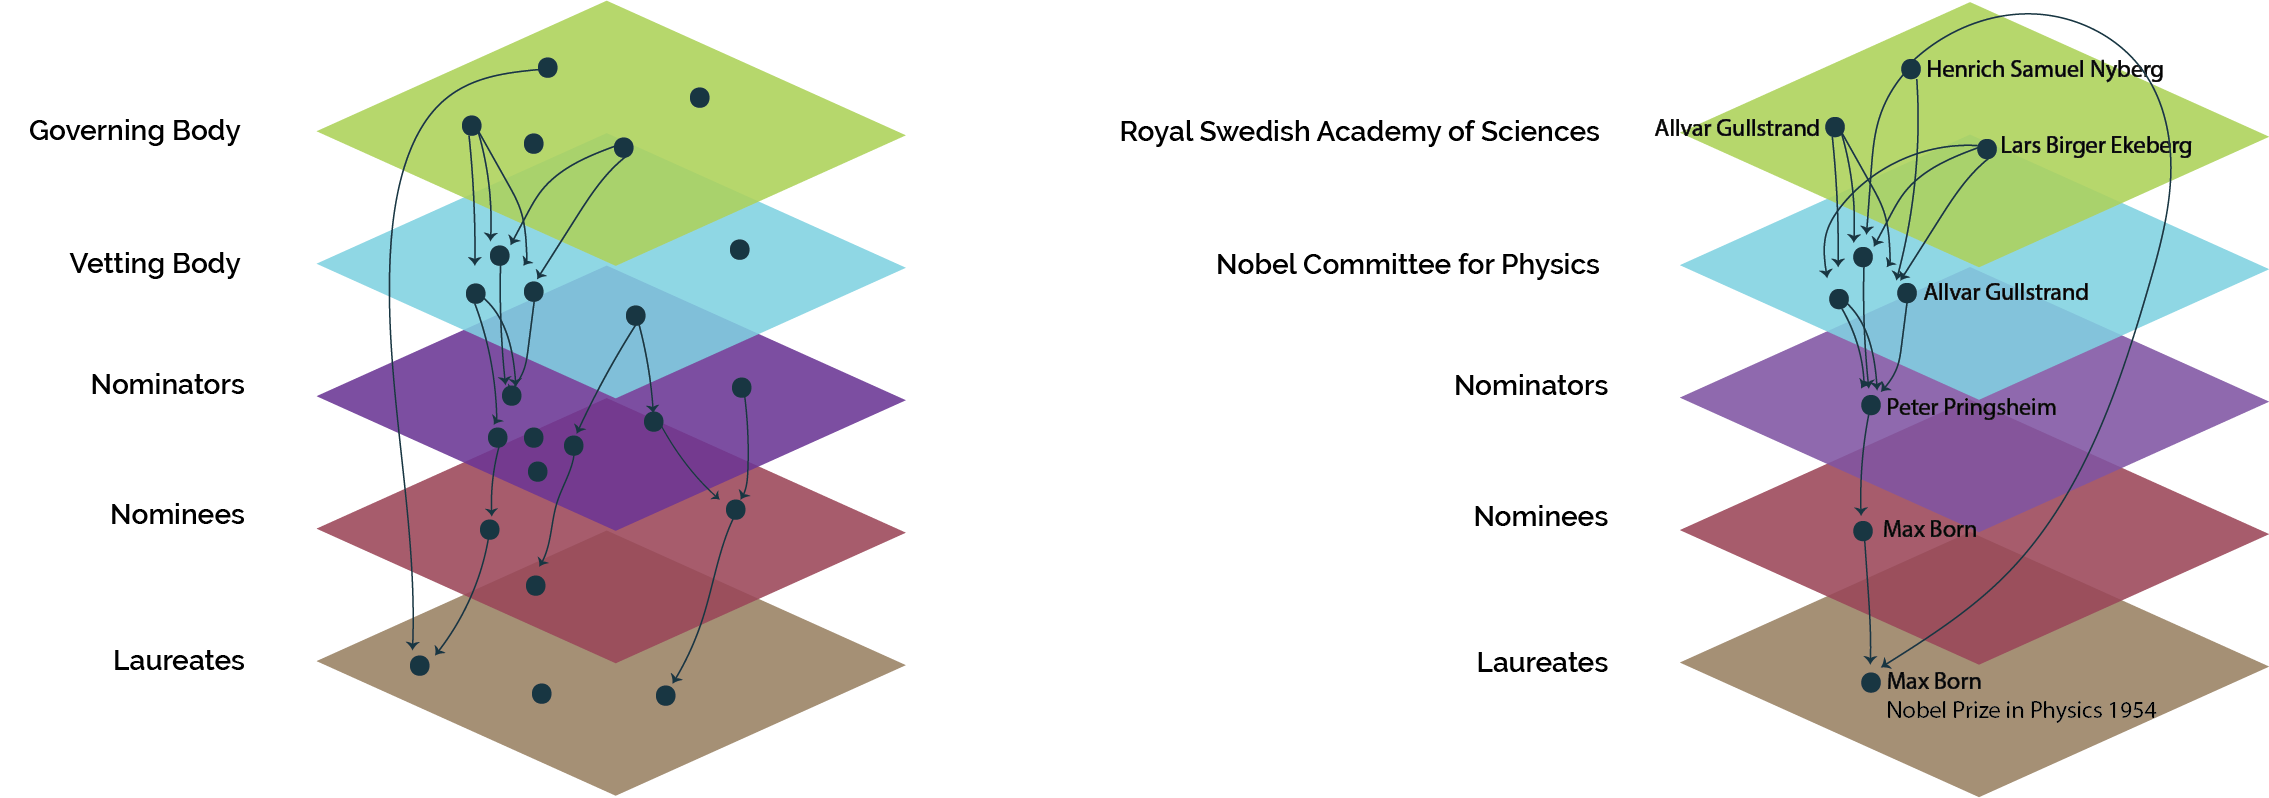
\includegraphics[width=\textwidth]{Fig1.png}
\caption{Multilayer network modeling framework for Nobel Prize selection. These are minimal schematic diagrams that include only a small subset of nodes and a small subset of the edges that actually exist between those nodes. More complete visualizations appear in Sec.~\ref{sec:results}. Left: Schematic of the five layers of our network as described in Sec.~\ref{sec:networkmodel}, namely, governing body, vetting body, nominators, nominees, and laureates. Nodes represent individuals and directed edges indicate decision-making power. That is to say, an edge pointing from person A to person B indicates that A was one of the people responsible for selecting B. The schematic at right is a (partial) example of the Nobel Prize in Physics from 1958. For the physics prize, the governing body is the Royal Swedish Academy of Sciences and the vetting body is the Nobel Committee for Physics; see Table~\ref{Tab1}.\label{Fig1}}
\end{figure*}

In constructing the prize selection network, we must keep in mind the various complexities of data. For instance, trivially, any laureate must also appear as a nominee. But beyond that, individuals may serve in multiple other roles, potentially in different years and for different prizes. For example:
\begin{itemize}
\item Willem Einthoven won the Nobel Prize in Physiology or Medicine in 1924 and nominated others for that same prize in 1901, 1905, 1917, and 1921.
\item Marie Curie was nominated for the Nobel Prize in Physics in 1902 and 1903, winning it in the latter year. She nominated other individuals for this prize in 1905 and 1910. Additionally, she was nominated for the Nobel Prize in Chemistry in 1911 and won it.
\item Bj{\o}rnstjerne Bj{\o}rnson was one of the original members of the Nobel Peace Prize vetting/selection body, the Norwegian Nobel Committee, from 1901 through 1906. He nominated other individuals for that prize in 1902, 1903, and 1907.  He himself was nominated for the Nobel Prize in Literature in 1902 and 1903, winning it during the second year.
\end{itemize}

To capture complexities like the aforementioned ones, we keep track of our data in the following manner. We represent each unique individual as a node. We attach to that node any personal demographics that are not directly tied to prize selection, such as gender, nationality, and so forth. Then, we apply edges to capture the roles of these individuals across prizes and across time. More specifically, each edge carries with it not just the specification of two nodes, but also a year, a Nobel Prize, and two network layers. For example, take the case of Marie Curie above. One of Curie's nominators for the Chemistry Prize in 1911 was Gaston Darboux. Therefore, our network has a directed edge pointing from Darboux to Curie. That edge specifies the year 1911, the field of chemistry, and the two network layers of nominators and nominees. Since Curie nominated Joseph Thomson for the Nobel Prize in Physics in 1905, the network has an edge pointing from Curie to Thomson. That edge specifies the year 1905, the field of physics, and, again, the two network layers of nominators and nominees.

\subsection{Data Acquisition}
\label{sec:dataacquisition}

There is no single source from which one can obtain all of the data necessary to construct the network model. We gather the necessary data for the five layers from a variety of sources, summarized in Table~\ref{tab2}. While information about governing bodies, vetting bodies, and laureates is available up through the present day, information about nominators and their nominees is made public only 50 years after the fact, subject to a secrecy rule imposed by the Nobel Foundation. All data gathering was performed programmatically in R using a reproducible pipeline of eight scripts, available in a public repository \citep{nobelgithub}. Below we describe each stage in sufficient detail for independent replication.

There are two broad steps to assembling the data. First, we must determine the identities of the individuals in each network layer and when they served. Then we must determine the relevant characteristics of those individuals, such as personal demographics. For the first step, we use the sources listed in the final column of Table~\ref{tab2}. For the second step, we use Wikidata \citep{wikidata}, a structured open knowledge database that, among other roles, provides the structured data behind many Wikipedia pages. By using Wikidata as our source for individual characteristics, we implicitly adopt the choices made by its contributors. As merely one example, we ourselves do not weigh in with inferences of individuals' gender; we use the gender data vetted by Wikidata, recognizing that any demographic data that is not self-identified is imperfect. Throughout the pipeline, we use Wikidata QIDs (unique entity identifiers of the form Q followed by a number) as the canonical identifier for each individual, enabling cross-referencing across data sources.

\begin{table}[t!]
\begin{tabular}{lll}
\textbf{Network Layer(s)}     & \textbf{Body}                       & \textbf{Source}                                                                                                                                    \\ \hline
                              &                                     &                                                                                                                                                    \\
Governing Body/Selection Body & Royal Swedish Academy of Sciences   &  \citet{wikidata}   \\
                              & Karolinska Institutet               &   \citet{KarolinskaEmployees}             \\
                              & Swedish Academy                     &  \citet{Ledamotsregister}                 \\
                              & Storting                            & \citet{wikidata}                          \\
                              &                                     &                                                                                                                                                    \\
Vetting Body                  & Nobel Committee for Chemistry       & \citet{NobelCommitteeChemistry}  \\
                              & Nobel Committee for Physics         &  \citet{NobelCommitteePhysics}   \\
                              & Nobel Committee for Physio/Med &  \citet{NobelCommitteePhysiology}             \\
                              & Nobel Committee for Literature      &   \citet{Ledamotsregister}              \\
                              & Norwegian Nobel Committee           &  \citet{NorwegianNobelCommittee}                  \\
                              &                                     &                                                                                                                                                    \\
Nominators                    &                                     & \citet{NobelPrizeWebsite}                                                  \\
                              &                                     &                                                                                                                                                    \\
Nominees                      &                                     & \citet{NobelPrizeWebsite}                                               \\
                              &                                     &                                                                                                                                                    \\
Laureates                     &                                     & Nobel Prize API v2.1                                                                                                                                           \\ \hline
\end{tabular}
\caption{Sources for the data in each network layer.\label{tab2}}
\end{table}

\subsubsection{Governing Bodies}
\label{sec:data-governing}

\textbf{Royal Swedish Academy of Sciences (RSAS).} The RSAS awards the prizes in Physics and Chemistry. Members are elected for life; their service begins at induction and ends at death. We scraped the membership list from the Swedish-language Wikipedia page \emph{Lista \"over ledam\"oter av Kungliga Vetenskapsakademien} \citep{Ledamotsregister}, which organizes members chronologically under bold year headers followed by bulleted lists of hyperlinked member names. Founding members (1739) appear under the headings ``Akademiens grundare'' and ``\"Ovriga.'' We parsed the rendered HTML by iterating through child elements in document order, updating the current induction year whenever a bold year header was encountered, and extracting all hyperlinked names from subsequent unordered lists. We excluded redlinks (articles not yet created) and non-article links.

Wikidata QIDs were resolved in batch using the MediaWiki \texttt{action=query\&prop=pageprops} API, which maps up to 50 Wikipedia page titles to their corresponding Wikidata items per request. This API also handles title normalization (e.g., converting underscores to spaces and resolving Unicode variants), which we accounted for when matching responses to input titles. We used exponential backoff (delay doubling from 2 seconds, up to 5 retries) for failed requests and imposed a 0.2-second delay between batches. For each member, we recorded the induction year as the start year; end years were left initially blank and later imputed from Wikidata death dates (see Section~\ref{sec:data-demographics}). Where multiple records existed for the same QID (e.g., due to class transfers within the Academy), we retained only the earliest induction record. The final dataset contains 2{,}312 RSAS members spanning 1739--2025, all with resolved QIDs.

\textbf{Swedish Academy.} The Swedish Academy awards the Prize in Literature. Its 18 members are appointed for life. We queried Wikidata directly via SPARQL, selecting all individuals holding position (P39) ``member of the Swedish Academy'' (Q207360), excluding honorary members (Q97563901). Start and end dates were extracted from the \texttt{pq:P580} and \texttt{pq:P582} qualifiers on each position statement and parsed from Wikidata's ISO~8601 datetime format (e.g., \texttt{1871-12-20T00:00:00Z} $\to$ 1871). All SPARQL queries throughout the pipeline were executed via HTTP POST to the Wikidata Query Service endpoint, with results returned in JSON format. We implemented retry logic with exponential backoff (5-second base delay, up to 10 retries) and identified our bot with a descriptive User-Agent string per Wikidata's access policy. The query yielded 202 member records.

\textbf{Storting (Norwegian Parliament).} The Storting awards the Peace Prize. We queried Wikidata for all entities classified as human (P31 = Q5) holding position (P39) ``member of the Storting'' (Q9045502), extracting start and end dates from position qualifiers. Norwegian parliamentarians may serve non-consecutive terms; we consolidated consecutive terms by grouping each member's service periods chronologically and merging periods where the gap between one term's end year and the next term's start year was at most one year. Non-consecutive terms were preserved as separate records. This yielded 4{,}281 member-term records spanning 1814--2025.

\textbf{Karolinska Institutet.} The Karolinska Institutet (KI) awards the Prize in Physiology or Medicine. Prior to 1977, all full professors at KI constituted the selection body; in 1977 the Nobel Assembly was established as a distinct entity, and in 1984 its membership was fixed at 50. Neither Wikidata nor KI's website publishes a complete roster of the Nobel Assembly.

We compiled KI professor data from Project Runeberg's digitized editions of the Swedish state calendar (\emph{statskalendern}) \citep{KarolinskaEmployees}, covering 1881--1970. Fourteen editions were manually mined for each professor's name, start year, and end year. Separately, Wikidata QIDs were searched and connected to each individual, verifying that biographical information matched or was plausible. The resulting spreadsheet contains one row per professor; we retained the 140 records with confirmed QIDs and both start and end years.

Post-1970 Nobel Assembly membership is not publicly available: Wikidata contains essentially no position (P39) or membership (P463) records for the Nobel Assembly entity (Q3375124), KI's website does not publish a member roster, and Project Runeberg's digitized calendars stop circa 1972. This is a known structural gap in our data (see Section~\ref{sec:gaps}).

\subsubsection{Vetting Bodies (Nobel Committees)}
\label{sec:data-vetting}

Each prize has a dedicated Nobel Committee that reviews nominations and prepares recommendations for the governing body.

\textbf{Chemistry, Physics, and Physiology/Medicine Committees.} These three committees are documented on Swedish-language Wikipedia \citep{NobelCommitteeChemistry,NobelCommitteePhysics,NobelCommitteePhysiology}. We extracted membership lists using a general-purpose parser that fetches wikitext (not rendered HTML) via the MediaWiki API (\texttt{action=parse\&prop=wikitext}), splits the text into sections by heading markers, and extracts bullet-list entries from sections titled ``Tidigare ledam\"oter'' (former members), ``Nuvarande ledam\"oter'' (current members), and ``Sekreterare'' (secretaries). Each entry follows one of several Swedish Wikipedia conventions: \texttt{[[Name]], YYYY--YYYY} (former members with date range), \texttt{[[Name]], invald YYYY} (current members, Swedish format), or \texttt{[[Name]], YYYY--} (current members, open-ended). We parsed Wikipedia article titles from double-bracket link syntax, extracted start and end years via regular expressions, and resolved QIDs through the batch MediaWiki API. The Swedish Wikipedia page for the Physiology/Medicine committee explicitly states ``Listan \"ar ofullst\"andig'' (the list is incomplete). Final counts: Chemistry 50 members, Physics 51, Physiology/Medicine 72 (59 with QIDs).

\textbf{Literature Committee.} The Nobel Committee for Literature is drawn from the Swedish Academy. No standalone membership list exists on Wikipedia. Instead, we extracted committee service years from individual member biographies on \texttt{svenskaakademien.se} \citep{Ledamotsregister}. We first queried Wikidata for all Swedish Academy members with their seat numbers (extracted from position labels matching the pattern ``member of the Swedish Academy at seat $N$''). We then constructed biography page URLs following the site's convention: \texttt{/de-aderton/stol-nr-\{seat\}-\{name-slug\}}, where the name slug is a lowercased, hyphen-separated, ASCII-transliterated version of the member's name.

The Swedish Academy website is built as a Nuxt.js single-page application. Rather than executing JavaScript, we extracted biography text directly from the \texttt{\_\_NUXT\_DATA\_\_} script tag embedded in each page's HTML source. This payload contains HTML-encoded biography text; we decoded HTML entities, stripped markup tags, and searched for mentions of ``Nobelkommitt\'en'' followed by year ranges. Two-digit years were expanded to four digits based on context (e.g., ``1969--86'' $\to$ 1969--1986). We retained only members whose biographies mentioned Nobel Committee service, yielding 35 members. This extraction method is fragile to future website redesigns.

\textbf{Norwegian Nobel Committee.} The Norwegian Nobel Committee both vets nominations and awards the Peace Prize. We parsed the membership table from the English Wikipedia page \emph{List of members of the Norwegian Nobel Committee} \citep{NorwegianNobelCommittee}, extracting start and end years and resolving QIDs via the batch MediaWiki API. This yielded 61 members (57 with QIDs).

\subsubsection{Nominations}
\label{sec:data-nominations}

We scraped the Nobel Prize Nomination Archive \citep{NobelPrizeWebsite}, which is subject to a 50-year secrecy rule. As of 2025, nomination records are available through 1974 or 1975 for Physics, Chemistry, Literature, and Peace. Physiology or Medicine nominations are available only through 1953; the Karolinska Institutet has not released records for 1954--1974, likely related to the 1977 Swedish transparency law and the concurrent restructuring that created the Nobel Assembly.

The archive's web interface uses numeric prize codes in its URL parameters: Physics = 1, Chemistry = 2, Physiology or Medicine = 3, Literature = 4, Peace = 5. For each of 353 prize-year combinations, we first retrieved the list page and extracted all nomination IDs from links to detail pages. We then scraped each detail page to extract the nomination year, prize category, and the names and internal person IDs of all nominees and nominators. Detail pages use a two-column table layout with bold section headers (``Nominee:'' and ``Nominator:'') followed by person links. We classified each person link by walking through all table cells in document order and tracking which section header was most recently encountered. A single nomination may list multiple nominees (16.3\% of nominations) and, more rarely, multiple nominators (1.1\%), reflecting joint nominations and co-signed nomination letters; we generated all pairwise nominee--nominator combinations.

Prize names were standardized to a common vocabulary (e.g., ``Physiology or Medicine'' $\to$ ``Physiology/Medicine''). The Peace Prize archive uses the header format ``Nomination for Nobel Peace Prize'' rather than ``Nobel Prize in \ldots'' as used by the other four categories; we handled this as a special case in parsing. List pages were fetched sequentially with 0.5-second inter-request delays; detail pages were fetched in parallel across $N-1$ CPU cores (capped at 12) with 0.2-second per-worker delays. Partial results were checkpointed to disk after each prize-year to allow resumption. The final dataset contains 27{,}932 nomination records spanning 22{,}600 unique nominations, 4{,}006 unique nominees, and 11{,}650 unique nominators. Among these, 755 records (2.7\%) have anonymous or unlisted nominators, and 2 records represent self-nominations.

\subsubsection{Laureates}
\label{sec:data-laureates}

We retrieved all Nobel Prize laureates from the official Nobel Prize API (v2.1, \texttt{api.nobelprize.org/2.1/laureates}), which provides structured JSON data including Wikidata QIDs, names, gender, award year, prize category, prize portion, motivation text, and primary affiliation at the time of award. We paginated through all results and filtered to the five original prize categories, excluding the Sveriges Riksbank Prize in Economic Sciences (established 1969). Laureates who received multiple prizes (7 individuals, including Marie Curie, Linus Pauling, Frederick Sanger, John Bardeen, and K.~Barry Sharpless) appear as separate records per prize. The final dataset contains 927 laureate-prize records representing 919 unique individuals, with 100\% QID coverage.

\subsubsection{Entity Resolution for Nomination Archive People}
\label{sec:data-entity-resolution}

The nomination archive identifies people by internal numeric IDs and names only, without Wikidata QIDs or other persistent identifiers. To integrate nomination data with the rest of the network (which uses Wikidata QIDs as the canonical identifier), we developed a two-stage matching procedure.

In the first stage, for each of the 14{,}471 unique people in the nomination archive, we scraped their detail page on \texttt{nobelprize.org}, extracting last name, first name, gender, birth year, and death year from labeled table cells. Scraping was parallelized across available cores in chunks of 500, with partial results checkpointed to disk. Of the 14{,}471 people, 4{,}571 (31.6\%) had birth years recorded; the remaining 9{,}903 (68.4\%) lacked birth year data entirely, rendering them unmatchable through our disambiguation strategy. Six records contained non-standard gender codes in the source database; we verified the identities of all six individuals by first name and confirmed they are male, recoding accordingly. One record had a transposed death year (1886 instead of 1986), which was corrected manually.

In the second stage, for each person with both a name and birth year (4{,}571 matchable individuals), we searched the Wikidata entity search API (limited to 10 candidates per query) and then verified each candidate's birth year via the Wikidata claims API (property P569, date of birth). A match was accepted only when the candidate's Wikidata birth year exactly equaled the birth year recorded in the Nobel archive. We did not attempt fuzzy name matching or approximate year matching, prioritizing precision over recall. This procedure matched 339 of 4{,}571 matchable individuals (7.4\%), representing 2.3\% of all nomination archive people. The low match rate reflects several factors: many early-twentieth-century nominators and nominees lack Wikidata entries; name transliterations between the archive's conventions and Wikidata's labels may differ; and our strict birth-year criterion rejects plausible matches where Wikidata records a different (or no) birth date. Unmatched individuals are represented in the network using temporary identifiers with a \texttt{NOM:} prefix (e.g., \texttt{NOM:7283}), preserving the nomination-layer topology even where cross-layer entity resolution was not possible.

\subsubsection{Demographic Enrichment}
\label{sec:data-demographics}

We fetched demographic attributes from Wikidata for all individuals with resolved QIDs across all data sources. The SPARQL query retrieved: English name label, gender (P21), country of birth (P19, traversed to sovereign state via P17), nationality (P27), birth date (P569), death date (P570), occupation (P106), and employer/institution (P108). Queries were executed in batches of up to 200 QIDs using the SPARQL \texttt{VALUES} clause, with individual fallback queries for any batch that failed. Multi-valued fields (nationality, occupation, institution) were collapsed into semicolon-delimited strings. Where multiple birth or death dates existed for a single QID (e.g., due to conflicting Wikidata sources), we retained the first non-missing value. After the initial demographic fetch for governing body, vetting body, and laureate QIDs, we performed a second pass to fetch demographics for the 339 matched nomination archive people, then re-collapsed all records to produce a single row per QID.

As a post-processing step, we imputed end-of-service years for RSAS members (who serve for life) using Wikidata death years. Of 2{,}312 RSAS members, 1{,}868 received imputed end years; 444 remain without end years (likely living members or individuals with unknown death dates). The final demographics table contains 7{,}221 unique individuals.

\subsection{Network Construction}
\label{sec:network-construction}

The final network was assembled from all intermediate data files. Nodes correspond to unique individuals identified by Wikidata QIDs, with demographic attributes from Section~\ref{sec:data-demographics}. Edges are directed and carry metadata for year, prize category, and the layer identities of the source and target nodes. We defined five edge types reflecting the institutional flow of the selection process:

\begin{enumerate}
    \item \textbf{Governing body $\to$ vetting body.} For each vetting body member, we created edges from all governing body members who were active at the start of the vetting member's service. ``Active'' means the governing body member's start year is at or before the vetting member's start year, and the governing body member's end year (if known) is at or after the vetting member's start year. The edge year is the vetting member's start year.

    \item \textbf{Vetting body $\to$ nominator.} For Chemistry, Physics, and Physiology/Medicine, Nobel Committees solicit nominations from qualified individuals. For each prize-year, we created edges from all active vetting body members to all nominators who submitted nominations that year.

    \item \textbf{Nominator $\to$ nominee.} Direct edges from each nominator to each nominee within a nomination record. For nominations with multiple nominees or nominators, all pairwise combinations were generated. Edges were deduplicated.

    \item \textbf{Governing body $\to$ laureate.} For Chemistry, Physics, Physiology/Medicine, and Literature, we created edges from all governing body members active in the award year to the laureate.

    \item \textbf{Vetting body $\to$ laureate.} For Peace only, the Norwegian Nobel Committee both evaluates nominations and awards the prize. Edges connect active committee members in the award year to the laureate.
\end{enumerate}

The body-to-prize mappings are: RSAS $\to$ \{Chemistry, Physics\}; Karolinska Institutet $\to$ Physiology/Medicine; Swedish Academy $\to$ Literature; Storting $\to$ Peace. After deduplication, the network contains 7{,}221 nodes and 305{,}199 edges. Edge counts by type are: governing body $\to$ laureate (147{,}965; 48.5\%), vetting body $\to$ nominator (87{,}492; 28.7\%), governing body $\to$ vetting body (42{,}360; 13.9\%), nominator $\to$ nominee (26{,}654; 8.7\%), and vetting body $\to$ laureate (728; 0.2\%). Edge counts by prize are: Physics (121{,}290), Chemistry (111{,}622), Physiology/Medicine (49{,}060), Peace (15{,}853), and Literature (7{,}374). The lower counts for Physiology/Medicine reflect the Karolinska data gap post-1970 and the truncated nomination archive (through 1953 only); the lower count for Literature reflects the smaller Swedish Academy membership (18 seats).

The network contains 220 self-loops arising from individuals who occupy roles in multiple layers simultaneously: 148 governing $\to$ vetting edges where RSAS members also served on Nobel Committees; 44 governing $\to$ laureate edges where RSAS members subsequently won Nobel Prizes (e.g., Svante Arrhenius, Ernest Rutherford); 26 vetting $\to$ nominator edges where committee members also submitted nominations; and 2 nominator $\to$ nominee self-nominations. We retained all self-loops as they reflect genuine structural features of the selection process.

\subsection{Data Quality Assessment}
\label{sec:diagnostics}

We performed a comprehensive 42-point diagnostic audit of all intermediate and output data files. Table~\ref{tab:diagnostics} summarizes the key results. Below we discuss findings organized by data source and assess the overall fitness of the dataset for network analysis.

\begin{table}[t!]
\footnotesize
\centering
\caption{Summary of data quality diagnostics across all data sources. Checks are classified as passed (no issues) or warning (expected structural limitation or quality note).\label{tab:diagnostics}}
\bigskip
\begin{tabular}{lcc}
\textbf{Category} & \textbf{Checks Passed} & \textbf{Warnings} \\ \hline
File integrity & 9/9 & 0 \\
Governing bodies & 8/9 & 1 \\
Vetting bodies & 4/5 & 1 \\
Nominations & 3/4 & 1 \\
Entity resolution & 2/3 & 1 \\
Laureates & 3/5 & 2 \\
Demographics & 2/3 & 1 \\
Network structure & 4/8 & 4 \\ \hline
\textbf{Total} & \textbf{31/42} & \textbf{11} \\
\end{tabular}
\end{table}

\textbf{Governing bodies.} All four governing bodies achieved 100\% QID resolution. All year values fall within plausible historical ranges (1700--2026), and no records have start year exceeding end year (after correction of three RSAS records where death-year imputation produced anomalous end years; these were reverted to missing). Of 2{,}312 RSAS members, 444 (19.2\%) remain without end years after imputation, likely because they are still living or their death dates are not recorded in Wikidata. These members are treated as currently active when determining temporal overlap for edge construction.

\textbf{Vetting bodies.} QID completeness ranges from 81.9\% (Physiology/Medicine, reflecting the acknowledged incompleteness of its Swedish Wikipedia source) to 100\% (Chemistry, Physics, Literature). We cross-validated committee members against their parent governing bodies: 42 of 45 Chemistry committee members and 44 of 50 Physics committee members appear in the RSAS roster. Only 23 of 52 Physiology/Medicine committee members appear in the Karolinska roster, attributable to the Karolinska data covering only 1881--1970 while the committee list extends to 2025.

\textbf{Nominations.} All five prize categories are represented with year ranges matching expectations. All 27{,}932 records have nominee person IDs; 755 (2.7\%) lack nominator person IDs (anonymous or unlisted nominators).

\textbf{Entity resolution.} Of 14{,}474 unique people in the nomination archive, only 339 (2.3\%) were matched to Wikidata QIDs. The primary bottleneck is missing biographical data: 9{,}903 people (68.4\%) lack birth years, making Wikidata disambiguation infeasible. As a consequence, 21.4\% of all edge endpoints in the final network use unresolved \texttt{NOM:} prefix identifiers, and 35.4\% of edges involve at least one such identifier. These edges preserve the nomination-layer topology but cannot be linked to individuals in other layers.

\textbf{Laureates.} All 927 laureate-prize records have QIDs (100\% coverage), and all 919 unique QIDs appear in the nodes file. Of 919 laureates, 267 lack governing body $\to$ laureate edges: 139 are Peace laureates (expected, since Peace uses the vetting $\to$ laureate pathway) and 128 are Physiology/Medicine laureates awarded after 1970 (the Karolinska data gap).

\textbf{Demographics.} The demographics table contains 7{,}221 unique QIDs with no duplicates. Completeness rates are: name 99.8\%, gender 99.5\% (90.3\% male, 9.3\% female), birth country 78.7\%, nationality 97.2\%, birth year 99.5\%, death year 78.2\%, occupation 97.4\%, and institutional affiliation 38.4\%. No records have birth year exceeding death year, and 57 records with birth years prior to 1700 correspond to historically accurate early members of the RSAS (founded 1739) and Storting (founded 1814).

\textbf{Network structure.} No duplicate edges exist. Among edges with resolved QIDs on both endpoints, 4{,}624 nodes are involved, with mean degree 85.3, median degree 13, and maximum degree 1{,}159. A total of 2{,}466 nodes (34.2\%) are isolates; these are predominantly nomination archive people who were matched to Wikidata QIDs (and thus appear in the nodes table) but whose \texttt{NOM:} prefix identifiers in the edge list were not replaced, an artifact of the identifier resolution process rather than a true structural feature.

\subsubsection{Known Structural Gaps}
\label{sec:gaps}

We document seven structural limitations inherent to the available sources:
\begin{enumerate}
    \item \emph{Karolinska Institutet post-1970 gap.} Nobel Assembly membership after 1970 is not publicly available, resulting in missing governing body $\to$ laureate and governing body $\to$ vetting body edges for Physiology/Medicine after 1970.

    \item \emph{Nomination archive 50-year secrecy rule.} Nomination data are available through 1974--1975 for most prizes, but only through 1953 for Physiology/Medicine.

    \item \emph{Physiology/Medicine vetting body incompleteness.} The Swedish Wikipedia source for this committee is self-reportedly incomplete.

    \item \emph{Literature committee extraction fragility.} Committee service years were parsed from a Nuxt.js SPA payload, which may break if the Swedish Academy redesigns its website.

    \item \emph{Low nomination QID match rate.} Only 2.3\% of nomination archive people were matched to Wikidata, primarily because 68.4\% lack birth years.

    \item \emph{RSAS end-year imputation.} 19.2\% of RSAS members lack end years after death-year imputation and are treated as currently active, which may slightly overcount active members in recent years.

    \item \emph{Storting term consolidation.} Non-consecutive Storting terms are preserved, but gaps between terms may not perfectly reflect actual departure and return dates.
\end{enumerate}

\subsubsection{Fitness for Network Analysis}

Despite these gaps, the dataset is suitable for multilayer network analysis. The governing body and vetting body layers have high completeness (93--100\% QID resolution), and temporal coverage extends from each institution's founding to the present, with the notable exception of Karolinska post-1970. The laureate layer has 100\% QID coverage and spans 1901--2025. The nomination layer, while limited in entity resolution, preserves the full topological structure of nominator--nominee relationships through the \texttt{NOM:} identifier system; analyses that do not require cross-layer linking of nomination-layer individuals can use these edges directly. The primary analytical constraints are: (a)~Physiology/Medicine analyses are limited by the Karolinska gap and the truncated nomination archive; (b)~cross-layer analyses linking nominators or nominees to governing/vetting body members are limited by the 2.3\% QID match rate; and (c)~the 34.2\% isolate node rate is an artifact of identifier resolution rather than a true structural feature. Researchers should consider these constraints when designing analyses, particularly for prize-specific comparisons involving Physiology/Medicine.

\subsection{Network Analysis}

To do our analysis we use the \texttt{multinet} package in R \citep{MagRosVeg2021}.

Some possibly useful links:
\begin{itemize}
	\item \url{https://www.nature.com/articles/s41598-020-72626-y}
	\item \url{https://link.springer.com/article/10.1007/s10618-020-00716-6}
	\item \url{https://www.frontiersin.org/articles/10.3389/fnsys.2021.624183/full}
	\item \url{https://search.r-project.org/CRAN/refmans/multinet/html/Communities.html}
	\item \url{https://cs.paperswithcode.com/paper/community-detection-with-node-attributes-in#code}
	\item \url{https://paperswithcode.com/search?q_meta=&q_type=&q=community+detection+multilayer+}
\end{itemize}

\section{Results}
\label{sec:results}

\section{Discussion and Conclusions}
\label{sec:discussionandconclusions}

\bibliographystyle{plainnat}
\bibliography{bibliography}

\section*{Acknowledgments}

We are grateful to the Institute for Computational and Experimental Research in Mathematics (ICERM) where this project was begun as part of a program on Data Science and Social Justice.

\end{document}
